% 20-12(20쪽) — $\seg{BC}\parallel\seg{DE}$ 인 삼각형 ABC(원문 「오른쪽 그림」). 스캔 화질이 낮아 TikZ 로 다시 그림.
% 라벨은 원문에 있는 것만 — 꼭짓점 A·B·C·D·E, 길이 2·3, $\log_2 x$, $\log_2 y^2$.
% 평행 표시는 원문처럼 두 변 가운데의 화살표 꼴. 상수 $k$(답)는 그림에서 읽히지 않게 적지 않는다.
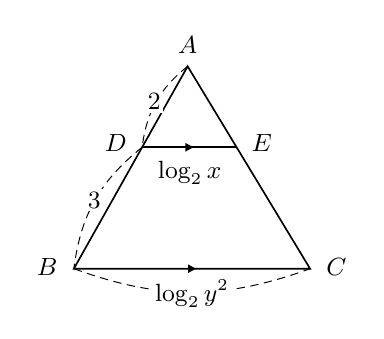
\begin{tikzpicture}[line width=0.6pt, x=1cm, y=1cm]
  \coordinate (A) at (1.445,2.57);
  \coordinate (B) at (0,0);
  \coordinate (C) at (3.0,0);
  \coordinate (D) at (0.867,1.542);
  \coordinate (E) at (2.067,1.542);
  \draw (A) -- (B) -- (C) -- cycle;
  \draw (D) -- (E);
  % 평행 표시(원문의 가운데 화살표)
  \fill (1.517,1.542) -- (1.417,1.597) -- (1.417,1.487) -- cycle;
  \fill (1.550,0) -- (1.450,0.055) -- (1.450,-0.055) -- cycle;
  % 길이 표시의 점선 호
  \draw[densely dashed, line width=0.35pt] (A) to[bend right=22] (D);
  \draw[densely dashed, line width=0.35pt] (D) to[bend right=22] (B);
  \draw[densely dashed, line width=0.35pt] (B) to[bend right=20] (C);
  \node[font=\small, anchor=south] at (1.445,2.60) {$\pt{A}$};
  \node[font=\small, anchor=east] at (-0.08,0.02) {$\pt{B}$};
  \node[font=\small, anchor=west] at (3.08,0.02) {$\pt{C}$};
  \node[font=\small, anchor=east] at (0.80,1.60) {$\pt{D}$};
  \node[font=\small, anchor=west] at (2.13,1.60) {$\pt{E}$};
  \node[font=\small, fill=white, inner sep=1pt] at (1.02,2.12) {$2$};
  \node[font=\small, fill=white, inner sep=1pt] at (0.26,0.87) {$3$};
  \node[font=\small, anchor=north] at (1.47,1.49) {$\log_2 x$};
  \node[font=\small, fill=white, inner sep=1pt, anchor=north] at (1.50,-0.10) {$\log_2 y^2$};
\end{tikzpicture}
